\begin{section}{背景}


    \textbf{图形神经网络}。GNN的目的是在一个具有节点表征
    $\textit{X}\in\textit{R}^{\vert\textit{V}\vert\times d}$
    的图上学习信号/特征的函数,其中$d$表示节点特征维度。对于典型的半监督节点分类任务~\cite{kipf2016semi},其中每个节点都与一个标签相关、 一个层的GNN 参数化为被训练来学习节点表征,这样可以被准确预测。GNN的训练过程实际上可以描述为基于\textit{消息传递机制}~\cite{gilmer2017neural}的节点表示学习。从分析上看,给定一个图和一个节点,GNN的第三层被定义为
    \begin{equation}
        \label{eq:gnn}
        \vspace{-1mm}
        \begin{split}
            \mathbf{h}_{v}^{(\ell+1)} &= \boldsymbol{f}_{\boldsymbol{\theta}}^{(\ell+1)} \bigg(\mathbf{h}_{v}^{(\ell)}, \big\{\!\!\big\{ \mathbf{h}^{(\ell)}_u  \big\}\!\!\big\}_{u \in \mathcal{N}(v)} \bigg) \\
            &= \Psi^{(\ell+1)}_{\boldsymbol{\theta}}\bigg( \mathbf{h}_{v}^{(\ell)},  \Phi^{(\ell+1)}_{\boldsymbol{\theta}}\Big(\big\{\!\!\big\{\mathbf{h}^{(\ell)}_u  \big\}\!\!\big\}_{u \in \mathcal{N}(v)}\Big) \bigg),
        \end{split}
        \vspace{-2mm}
        \end{equation}
    其中,$\textit{h}_{v}^{(\textit{l})}$表示节点$v$在$\ell$第三层的表示, $\textbf{h}^{(0)}_{v}$ 被初始化为 $\textbf{x}_{v}$($\textbf{X}$中第$v$行), $mathcal{N}(v)$表示节点$v$的邻居集合。
    GNN的每一层,即$\boldsymbol{f}_{\boldsymbol{\theta}}^{(\ell)}$,可以进一步分解为两个部分:
    1) 聚合函数$\Phi^{(\ell)}_{\boldsymbol{\theta}}$,它将节点$v$的邻居的节点表示作为输入,输出聚合的邻居表示。
    2) 更新函数$\Psi^{(\ell)}_{\boldsymbol{\theta}}$,它结合$v$的表示和聚集的邻域表示,为下一层更新节点$v$的表示。
    $\Phi^{(\ell)}_{\boldsymbol{\theta}}$和$\Psi^{(\ell)}_{\boldsymbol{\theta}}$都可以选择在不同类型的GNN中使用各种函数。
    为了在一台机器上训练GNN,我们可以在训练数据的整个图上使经验损失$\mathcal{L}(\boldsymbol{\theta})$最小化,即$\mathcal{L}(\boldsymbol{\theta}) = \vert\mathcal{V}\vert^{-1}\sum\nolimits_{v\in\mathcal{V}}。Loss\big(\mathbf{h}_{v}^{(L)},\mathbf{y}_{v}\big)$,
    其中$Loss(\cdot,\cdot)$表示损失函数(如交叉熵损失),$\mathbf{h}_{v}^{(L)}$表示来自GNN最后一层的节点$v$的表示。


    \textbf{GNN的分布式训练。} 分布式GNN训练首先将原始图划分为多个没有重叠的子图,这也可以被认为是小批。然后在不同的设备上并行地训练不同的小批。这里,Eq.~\ref{eq:gnn}可以进一步重新表述为
    \begin{equation}
\label{eq:mini-batch}
\vspace{-1mm}
\begin{split}
    \mathbf{h}_{v}^{(\ell+1)} = \boldsymbol{f}_{\boldsymbol{\theta}}^{(\ell+1)} \Big( \mathbf{h}_{v}^{(\ell)}, 
    &\underbrace{\big\{\!\!\big\{\mathbf{h}^{(\ell)}_u \big\}\!\!\big\}_{u \in  \mathcal{N}(v)   \cap \mathcal{S}(v)}}_{\text{In-subgraph nodes}} \\ &\cup \underbrace{\big\{\!\!\big\{\mathbf{h}^{(\ell)}_u  \big\}\!\!\big\}_{u \in \mathcal{N}(v) \setminus \mathcal{S}(v)}}_{\text{Out-of-subgraph nodes}}  \Big),
\end{split}
\vspace{-1mm}
\end{equation}

其中$\mathcal{S}(v)$表示节点$v$所属的子图。在本文中,我们考虑用多台本地机器和一台全球服务器对GNN进行分布式训练。原始输入图$\mathcal{G}$首先被划分为$M$子图,其中每个$\mathcal{G}_{m}(\mathcal{V}_{m},\mathcal{E}_{m})$代表第$m$子图。我们的目标是通过最小化每个局部损失,以分布式方式找到最佳参数集$\boldsymbol{\theta}$,即

\begin{equation}
    %\vspace{-2mm}
    \label{eq:distributed loss}
    \begin{split}
        \text{min}_{\boldsymbol{\theta}_{m}} & \;\mathcal{L}_{m}^{\text{Local}}\big(\boldsymbol{\theta}_{m}\big) = \frac{1}{\vert\mathcal{V}_m \vert}\sum_{v\in\mathcal{V}_m} Loss\big(\mathbf{h}_{v}^{(L)},\mathbf{y}_{v}\big), \\ & \text{s.t.}\quad\forall \;\;m=1,2,\cdots,M\;\; \text{\emph{in parallel}},
    \end{split}
\end{equation}

其中$\{\boldsymbol{\theta}_{m}\}_{m=1}^M$是每个本地GNN模型的参数,$\mathbf{h}_{v}^{(L)}$遵循Eq.~\ref{eq:mini-batch}递归。在每一轮通信中,每个局部参数都被汇总以更新全局参数,即$\boldsymbol{\theta}=AGG(\boldsymbol{\theta}_{1},\boldsymbol{\theta}_{2},\cdots,\boldsymbol{\theta}_{M})$。

现有的分布式GNN框架一般都试图在通信成本和信息损失之间找到一个最佳的平衡点。"基于分区 "的方法将经典分布式训练中现有的数据并行技术在\emph{i.i.d}数据上推广到图数据上,并享有最小的通信成本。具体来说,当前子图之外的邻居的嵌入(如Eq.~\ref{eq:mini-batch})被放弃。"基于传播 "的方法考虑使用每个子图的邻居节点的通信来满足GNN的邻居聚合。如公式~\ref{eq:mini-batch}所示,当前子图之外的邻居节点的表示在不同子图之间交换。然而,随着GNN模型的深入,参与邻居聚合过程的邻居数量呈指数级增长,这就是所谓的 邻居爆炸问题 \emph{neighborhood explosion}。

然而,上述想法的一个潜在问题是嵌入的呆滞性,这意味着在前向传递过程中节点嵌入的延迟,反过来导致后向传递过程中梯度的延迟。这两种延迟都会损害模型的性能和收敛性。

\begin{figure*}[t!]
    \begin{center}
      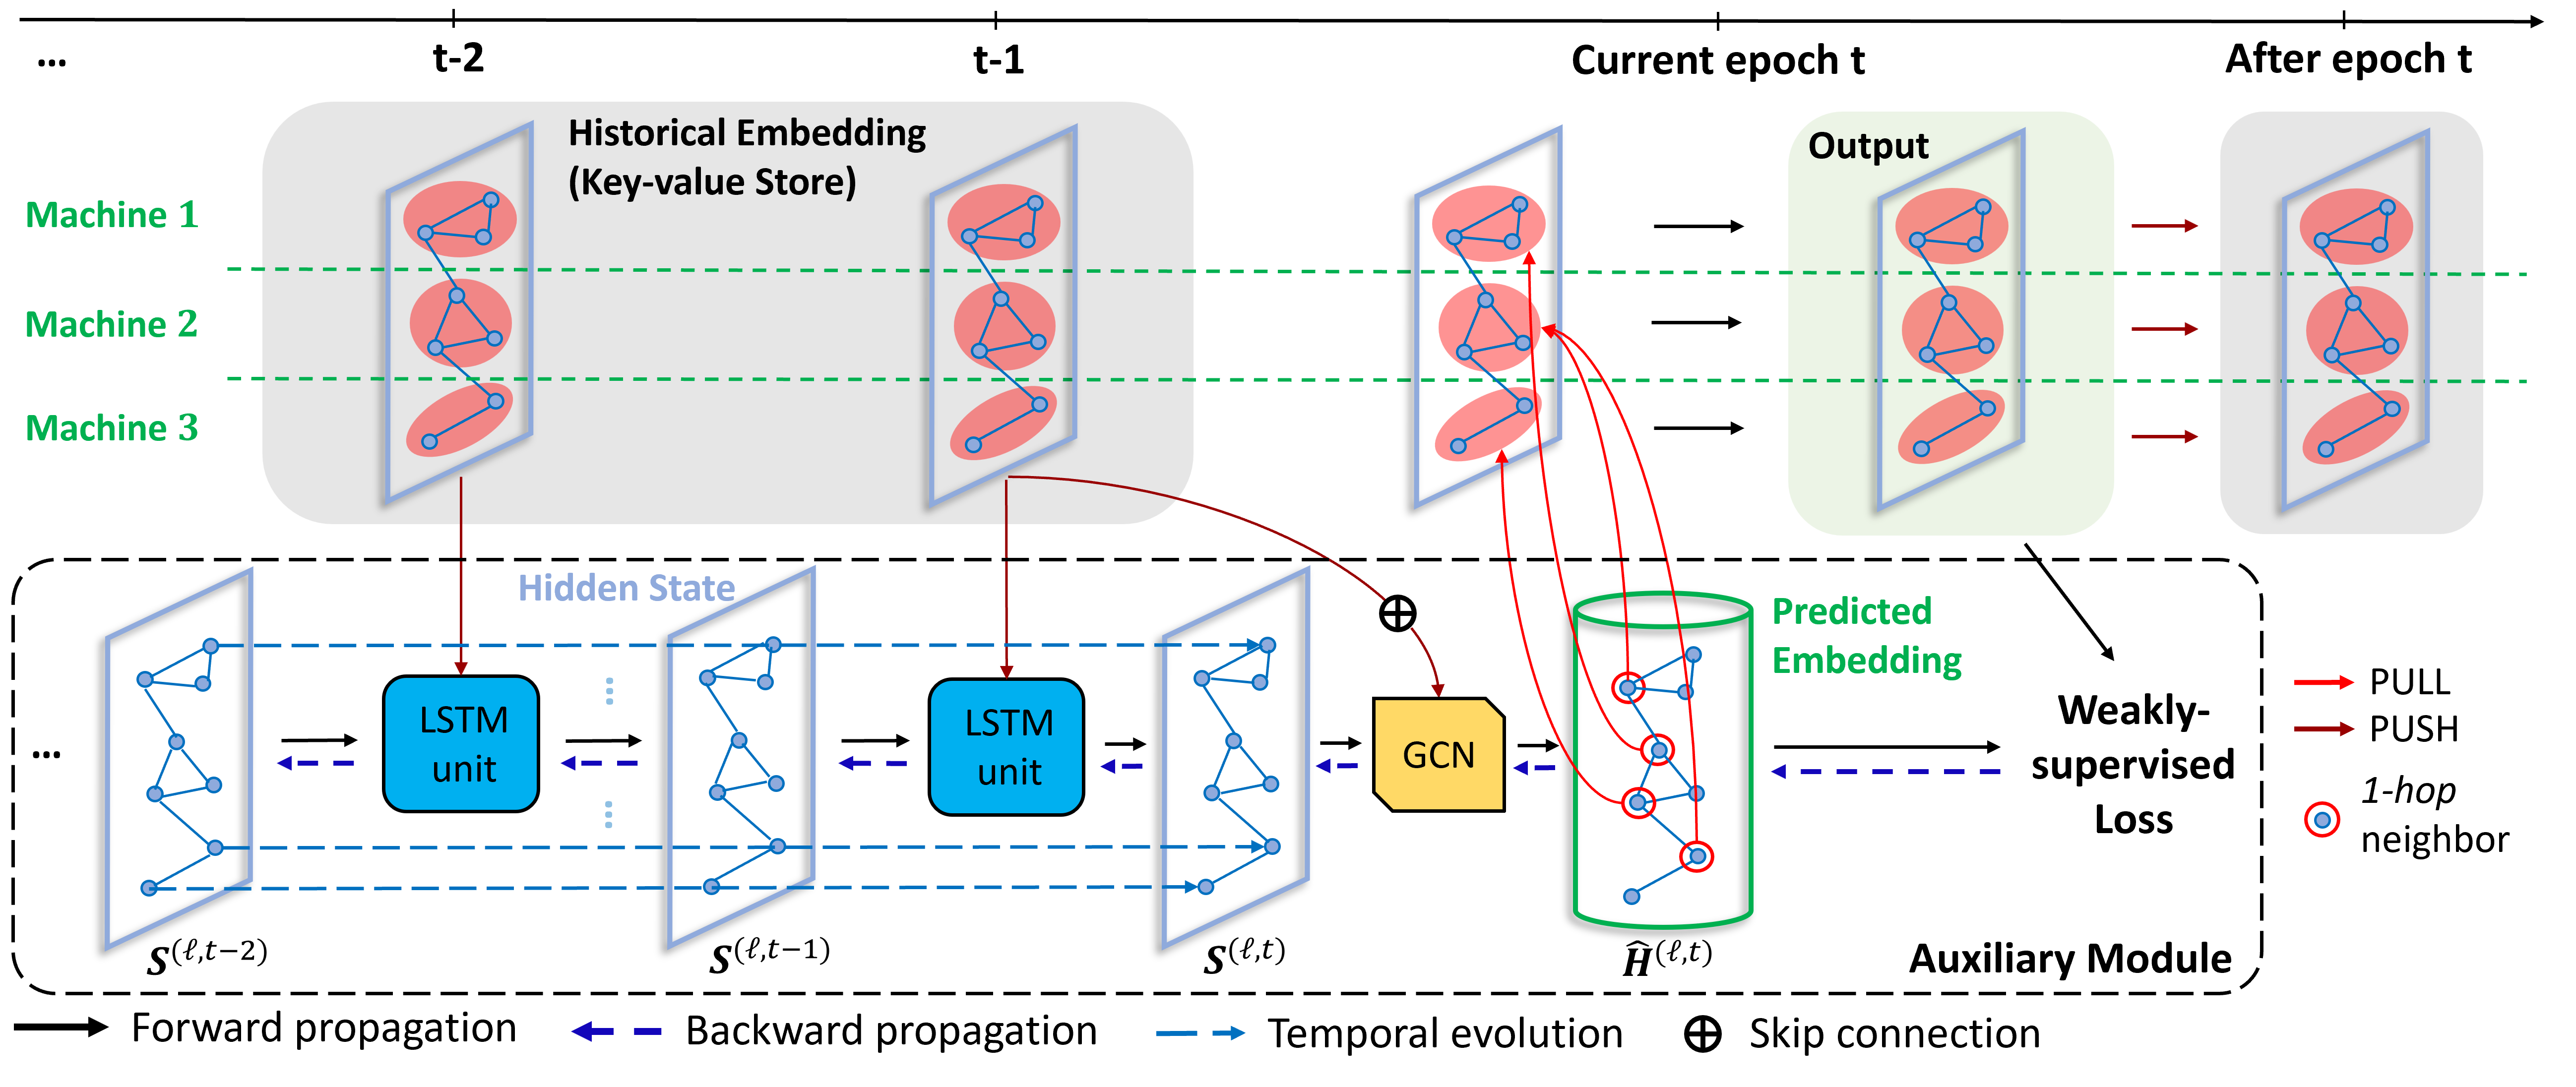
\includegraphics[width=0.95\textwidth]{figures/architecture.png}
    \end{center}
    \vspace{-4mm}
    \caption{A high level overview of our framework (per-layer view). Best viewed in color.}
    \label{fig:framework demo}
    \vspace{-3mm}
  \end{figure*}
\end{section}

